\section{Main results}
\label{sec:results}

% Remaster, 3 October 2026.  Main results = the three harnesses on
% TabReD against the published methods, on MLAgentBench head to head, on the
% case studies, and their cost.  Each subsection ends with a one-sentence
% Finding.  Ablations are in Section~\ref{sec:ablations}.

\subsection{TabReD: the harnesses among the tuned methods}
\label{sec:leaderboard}

Figure~\ref{fig:leaderboard} places the three harnesses among
the eighteen published methods; Table~\ref{tab:leaderboard} gives the raw
values. AutoDS-Tools reaches a mean normalised score of $\nAutoDS$, on par
with tuned LightGBM and below tuned XGBoost ($\nXGB$) and the strongest
published method, an MLP-PLR ensemble ($\nBest$). It is ahead of Terminus-2
($\nTerminus$) on \stshipAutoDSvsTerminusWins{} of 8 tasks.

\begin{figure*}[t]
\centering
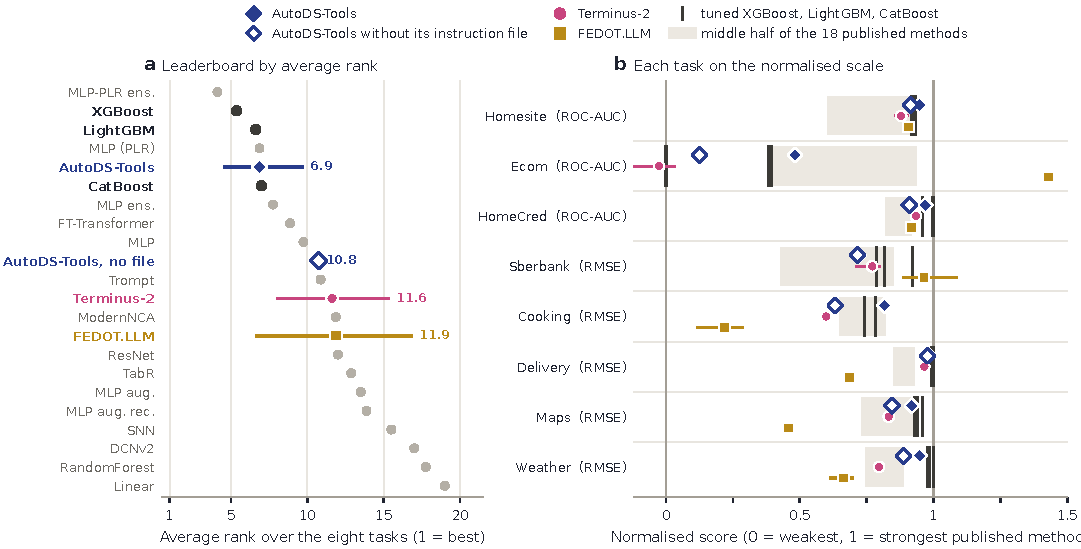
\includegraphics[width=\textwidth]{figures/fig_leaderboard.pdf}
\caption{The three harnesses among the eighteen tuned TabReD methods.
(a)~Average rank over the eight tasks; whiskers are 95\% bootstrap
intervals over tasks. (b)~Each task on the normalised scale; whiskers span
the three attempts. AutoDS-Tools is shown with its instruction file (filled) and
without it (open).}
\label{fig:leaderboard}
\end{figure*}
\begin{table*}[t]
\centering
\caption{Agent architectures placed in the TabReD leaderboard: full official temporal splits, the benchmark's metrics in raw units. Published rows are Optuna-tuned means over 15 seeds \citep{rubachev2024tabred}; agent rows use \texttt{gemma-4-31b-it}; agent rows are means over three attempts. Best per column in bold.}
\label{tab:leaderboard}
\small
\setlength{\tabcolsep}{3pt}
\begin{tabular}{lrrrrrrrrr}
\toprule
& \multicolumn{3}{c}{ROC-AUC $\uparrow$} & \multicolumn{5}{c}{RMSE $\downarrow$} & \\
\cmidrule(lr){2-4}\cmidrule(lr){5-9}
Method & Homesite & Ecom & HomeCred & Sberbank & Cooking & Delivery & Maps & Weather & Avg.\ rank \\
\midrule
\addlinespace[2pt]
\multicolumn{10}{l}{\itshape GBDT} \\
XGBoost & 0.9601 & 0.5763 & \textbf{0.8670} & 0.2419 & 0.4823 & 0.5468 & 0.1616 & 1.4671 & 5.4 \\
LightGBM & 0.9603 & 0.5758 & 0.8664 & 0.2468 & 0.4826 & 0.5468 & 0.1618 & \textbf{1.4625} & 6.6 \\
CatBoost & 0.9606 & 0.5596 & 0.8621 & 0.2482 & 0.4823 & \textbf{0.5465} & 0.1619 & 1.4688 & 7.0 \\
RandomForest & 0.9570 & 0.5764 & 0.8269 & 0.2640 & 0.4884 & 0.5959 & 0.1653 & 1.5838 & 17.8 \\
Linear & 0.9290 & 0.5665 & 0.8168 & 0.2509 & 0.4882 & 0.5579 & 0.1709 & 1.7679 & 19.0 \\
\addlinespace[2pt]
\multicolumn{10}{l}{\itshape Tabular DL} \\
MLP & 0.9500 & 0.6015 & 0.8545 & 0.2508 & 0.4820 & 0.5504 & 0.1622 & 1.5470 & 9.8 \\
SNN & 0.9492 & 0.5996 & 0.8551 & 0.2858 & 0.4838 & 0.5544 & 0.1651 & 1.5649 & 15.5 \\
DCNv2 & 0.9392 & 0.5955 & 0.8466 & 0.2770 & 0.4842 & 0.5532 & 0.1672 & 1.5782 & 17.0 \\
ResNet & 0.9469 & 0.5998 & 0.8493 & 0.2743 & 0.4825 & 0.5527 & 0.1625 & 1.5021 & 12.0 \\
FT-Transformer & 0.9622 & 0.5775 & 0.8571 & 0.2440 & 0.4820 & 0.5542 & 0.1625 & 1.5104 & 8.9 \\
MLP (PLR) & 0.9621 & 0.5957 & 0.8568 & 0.2438 & 0.4812 & 0.5527 & 0.1616 & 1.5177 & 6.9 \\
Trompt & 0.9588 & 0.5803 & 0.8355 & 0.2509 & 0.4809 & 0.5519 & 0.1624 & 1.5187 & 10.9 \\
\addlinespace[2pt]
\multicolumn{10}{l}{\itshape Ensembles} \\
MLP ens. & 0.9503 & 0.6019 & 0.8557 & 0.2447 & 0.4815 & 0.5494 & 0.1620 & 1.5186 & 7.8 \\
MLP-PLR ens. & \textbf{0.9629} & 0.5981 & 0.8585 & \textbf{0.2381} & \textbf{0.4806} & 0.5518 & \textbf{0.1612} & 1.4953 & 4.1 \\
\addlinespace[2pt]
\multicolumn{10}{l}{\itshape Training methodologies} \\
MLP aug. & 0.9523 & 0.6011 & 0.8449 & 0.2659 & 0.4832 & 0.5532 & 0.1631 & 1.5193 & 13.5 \\
MLP aug. rec. & 0.9531 & 0.5960 & 0.7453 & 0.2515 & 0.4834 & 0.5541 & 0.1636 & 1.5160 & 13.9 \\
\addlinespace[2pt]
\multicolumn{10}{l}{\itshape Retrieval-augmented} \\
TabR & 0.9487 & 0.5943 & 0.8501 & 0.2820 & 0.4828 & 0.5514 & 0.1639 & 1.4666 & 12.9 \\
ModernNCA & 0.9514 & 0.5765 & 0.8531 & 0.2593 & 0.4825 & 0.5498 & 0.1625 & 1.5062 & 11.9 \\
\midrule
\multicolumn{10}{l}{\itshape Agentic AutoML systems (this work)} \\
Terminus-2 \emph{(open harness)} & 0.9588 & 0.5585 & 0.8590 & 0.2491 & 0.4837 & 0.5482 & 0.1628 & 1.5247 & 11.6 \\
AutoDS-Tools \emph{(multi-agent)} & 0.9611 & 0.5800 & 0.8633 & 0.2515 & 0.4820 & 0.5474 & 0.1620 & 1.4783 & 6.9 \\
FEDOT.LLM \emph{(rigid pipeline)} & 0.9597 & \textbf{0.6200} & 0.8569 & 0.2398 & 0.4867 & 0.5620 & 0.1664 & 1.5651 & 11.9 \\
\bottomrule
\end{tabular}
\end{table*}


FEDOT.LLM ($\nFedot$) behaves differently from both agents. Its backend
search gives the best ROC-AUC of any method on \texttt{ecom-offers}
($\fedotEcomAuc$), and the same backend ranks 18th to 20th of 21 on four
regression tasks. Section~\ref{sec:ablations} shows how much of the
AutoDS-Tools lead comes from its instruction file.

\paragraph{Finding 1} With its instruction file, AutoDS-Tools is on par with tuned LightGBM
and ahead of Terminus-2 on \stshipAutoDSvsTerminusWins{} of 8 tasks
($p=\stshipAutoDSvsTerminusP$). FEDOT.LLM matches Terminus-2 on average and
differs from it on single tasks in both directions. None of the three reaches tuned XGBoost or the
strongest published method in this comparison.

\subsection{MLAgentBench: two harnesses from a working script}
\label{sec:mlab}

Table~\ref{tab:mlab} compares Terminus-2 with AutoDS-Tools on the eight
MLAgentBench tasks that repeat on our hardware, under one job, one verifier
and three attempts per task; AutoDS-Tools is shown with and without its
instruction file, and the comparison between harnesses uses the column
without it, since Terminus-2 carries none. AutoDS-Tools is the more accurate
of the two, taking \headWinsAutoDS{} of \headTasks{} tasks against
\headWinsTerminus{} for Terminus-2, with two ties: one task at the floor of
its metric and one inside the 5\% margin the table uses. Terminus-2 is the
faster and the less reliable: it uses about a third of the mean wall-clock
per trial, reaches its agent budget once in 24 trials where AutoDS-Tools
reaches it 13 times in 30 (the 30 include the two tasks that could not be
repeated), and ends without a submission in \headMissTerminus{} of 24
attempts against \headMissAutoDS{}. The spread
within a cell is large on this benchmark (Section~\ref{sec:stats}), so only
the win count and the submission counts are read as results.
\begin{table*}[t]
\centering
\caption{AutoDS-Tools with and without its prescribed-knowledge layer, and Terminus-2, on the eight MLAgentBench tasks that repeat on our hardware: one job, one verifier, three attempts per task. Mean, min and max are over the attempts that submitted; a superscript gives the number of submitting attempts where it is below three, and \emph{none} means no attempt submitted. Bold marks the better of AutoDS-Tools without the layer and Terminus-2 where the margin exceeds $5\%$. $\Delta$ is the change in mean score with the layer, divided by the larger of the two means, positive where the layer helps.}
\label{tab:mlab}
\footnotesize
\setlength{\tabcolsep}{3pt}
\begin{tabular}{llrrrrrrrrrr}
\toprule
 & & \multicolumn{3}{c}{AutoDS-Tools, layer off} & \multicolumn{3}{c}{AutoDS-Tools, layer on} & \multicolumn{3}{c}{Terminus-2} & \\
\cmidrule(lr){3-5}\cmidrule(lr){6-8}\cmidrule(lr){9-11}
Task & Metric & mean & min & max & mean & min & max & mean & min & max & $\Delta$ \\
\midrule
\texttt{clrs} & Ptr. acc. $\uparrow$ & \textbf{0.3909} & 0.3204 & 0.4404 & \multicolumn{3}{c}{none} & 0.1397$^{2}$ & 0.1330 & 0.1464 & \multicolumn{1}{c}{--} \\
\texttt{ogbn-arxiv} & Accuracy $\uparrow$ & \textbf{0.3866} & 0.2237 & 0.4790 & 0.5069 & 0.4334 & 0.5573 & 0.1606 & 0.0597 & 0.2655 & +0.24 \\
\texttt{spaceship-titanic} & Accuracy $\uparrow$ & \textbf{0.8074} & 0.8022 & 0.8131 & 0.8108 & 0.8080 & 0.8131 & 0.6590 & 0.5859 & 0.7059 & 0.00 \\
\texttt{house-price} & MAE $\downarrow$ & \textbf{15\,894.8} & 15\,529.7 & 16\,600.8 & 16\,433.4 & 16\,162.0 & 16\,904.2 & 21\,594.8$^{2}$ & 19\,422.1 & 23\,767.4 & -0.03 \\
\texttt{identify-contrails} & Dice $\uparrow$ & 0.0022 & 0.0000 & 0.0040 & 0.0478 & 0.0149 & 0.1137 & 0.0000$^{2}$ & 0.0000 & 0.0000 & +0.96 \\
\texttt{amp-parkinsons} & SMAPE $\downarrow$ & 62.2787$^{2}$ & 58.2113 & 66.3461 & 86.4637 & 81.7768 & 90.0803 & 60.4999$^{1}$ & -- & -- & -0.28 \\
\texttt{feedback} & MCRMSE $\downarrow$ & 0.8261 & 0.5403 & 1.2569 & \multicolumn{3}{c}{none} & \textbf{0.5279}$^{2}$ & 0.4972 & 0.5586 & \multicolumn{1}{c}{--} \\
\texttt{fathomnet} & micro-F1 $\uparrow$ & 0.1435$^{2}$ & 0.1428 & 0.1442 & \multicolumn{3}{c}{none} & \textbf{0.2440} & 0.0844 & 0.3846 & \multicolumn{1}{c}{--} \\
\bottomrule
\end{tabular}
\begin{tablenotes}\footnotesize
\item \texttt{identify-contrails} is counted as a tie between AutoDS-Tools and Terminus-2: both cells sit at the floor of the metric, and its $\Delta$ divides one small number by another and is not read as a result. Without the layer AutoDS-Tools takes 4 of the eight tasks against Terminus-2 and Terminus-2 2. Median trial: $6.1$ minutes for Terminus-2 against $10.9$ for AutoDS-Tools without the layer; means $19.1$ against $63.2$. Terminus-2 reached its agent budget once in $24$ trials, AutoDS-Tools $13$ times in $30$.
\end{tablenotes}
\end{table*}


\paragraph{Finding 2} From a working script, AutoDS-Tools takes
\headWinsAutoDS{} of \headTasks{} tasks and Terminus-2 \headWinsTerminus{};
Terminus-2 is three times faster on average and leaves three times as many attempts
without a submission.

\subsection{Three scientific case studies}
\label{sec:cases}

Three published studies with an author-reported baseline were turned into
Harbor tasks (Figure~\ref{fig:cases}, top row). Maize grain yield in the
Genomes-to-Fields trials~\citep{kick2023yield} is predicted for
location-years the model has never seen, with the authors' own split. Exit
state of jobs on the Fugaku supercomputer~\citep{antici2025fdata} is
predicted from what the scheduler knows at submission time; a constant
predictor scores $\caseFdataFloor$. Glass-transition temperature of polymers
in OpenPoly~\citep{wang2025openpoly} is predicted from a PSMILES string.
F-DATA and OpenPoly use random 80/20 splits, so their author figures come
from a different split: close in the case of F-DATA, distant in the case of
OpenPoly, where the authors used their full dataset.

\begin{figure*}[t]
\centering
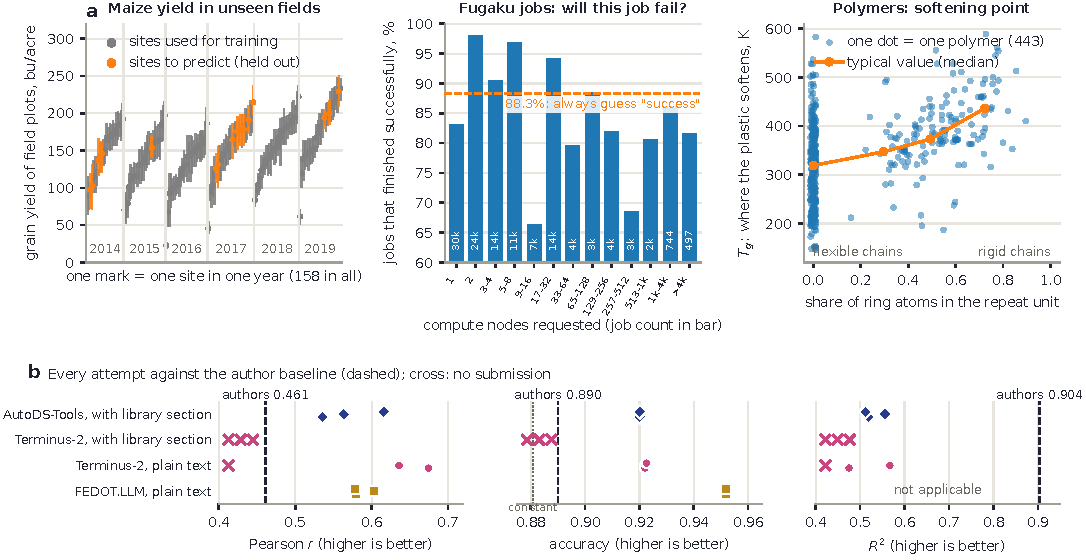
\includegraphics[width=0.96\textwidth]{figures/fig_cases.pdf}
\caption{The three case studies. Top: what each task asks, drawn from the
open data. Bottom: every attempt against the author baseline (dashed);
crosses mark attempts that ended without a submission.}
\label{fig:cases}
\end{figure*}

The task text was written for AutoDS-Tools and is the most prescriptive
condition in the paper: it names
LightAutoML~\citep{vakhrushev2021lightautoml} as the required library,
supplies a working snippet, lists the columns that leak the target,
describes the split and states the author baseline as the number to beat.
Every system has three attempts per case. AutoDS-Tools ran on that text
with its own instruction file off, since the text already names the library.
Terminus-2 ran on that text and on the same text with the library section
removed. FEDOT.LLM ran on the two tabular cases with a 40-minute backend
budget, its library being built in. Table~\ref{tab:cases} gives every row.
\begin{table*}[t]
\centering
\caption{Three scientific case studies, one row per system and task text: the published text with its library section, or the same text without it (plain). $n$ counts attempts that left a submission; mean, min and max are over those; minutes are the median agent time per attempt. Bold: the best system mean per case.}
\label{tab:cases}
\small
\setlength{\tabcolsep}{5pt}
\begin{tabular}{llllcrrrr}
\toprule
Case & Metric & System & Text & $n$ & mean & min & max & min/attempt \\
\midrule
Maize yield (G2F) & Pearson $r$ $\uparrow$ & \emph{authors} & & & 0.461 & & & \\
 & & AutoDS-Tools & with library section & 3/3 & 0.572 & 0.536 & 0.616 & 14.1 \\
 & & Terminus-2 & plain & 2/3 & \textbf{0.655} & 0.636 & 0.674 & 2.1 \\
 & & Terminus-2 & with library section & 0/3 & -- & -- & -- & 4.0 \\
 & & FEDOT.LLM & plain (library built in) & 3/3 & 0.587 & 0.578 & 0.603 & 52.8 \\
\midrule
Fugaku exit state (F-DATA) & Accuracy $\uparrow$ & \emph{authors} & & & 0.890 & & & \\
 & & AutoDS-Tools & with library section & 3/3 & 0.920 & 0.920 & 0.920 & 20.1 \\
 & & Terminus-2 & plain & 3/3 & 0.922 & 0.922 & 0.923 & 1.1 \\
 & & Terminus-2 & with library section & 0/3 & -- & -- & -- & 2.5 \\
 & & FEDOT.LLM & plain (library built in) & 3/3 & \textbf{0.952} & 0.952 & 0.952 & 45.4 \\
\midrule
Polymer $T_g$ (OpenPoly) & $R^2$ $\uparrow$ & \emph{authors} & & & 0.904 & & & \\
 & & AutoDS-Tools & with library section & 3/3 & \textbf{0.529} & 0.512 & 0.556 & 13.1 \\
 & & Terminus-2 & plain & 2/3 & 0.521 & 0.475 & 0.567 & 3.2 \\
 & & Terminus-2 & with library section & 0/3 & -- & -- & -- & 2.6 \\
\bottomrule
\end{tabular}
\begin{tablenotes}\footnotesize
\item AutoDS-Tools rows run the published text with the system's own instruction file off. FEDOT.LLM cannot act on the library section and has no molecular featurisation, so it has one row and was not run on OpenPoly. F-DATA: majority class scores 0.881. OpenPoly: the author figure is on the full dataset, ours on a subset with an 89-row test split, so that row is indicative only.
\end{tablenotes}
\end{table*}


Given the task text without the library section, Terminus-2 exceeded the
author baseline on maize (Pearson $r$ of $\caseTermPlainMaizeMin$ and
$\caseTermPlainMaizeMax$ against $\caseAuthorMaize$) and the author figure on
F-DATA ($\caseTermPlainFdataMean$ accuracy against $\caseAuthorFdata$), with
one to five minutes per attempt. On OpenPoly it chose RDKit~\citep{rdkit}
fingerprints and descriptors under XGBoost, the featurisation the authors
published.

With the library section in the text, Terminus-2 ended all
\caseTermPrescTotal{} attempts without a submission, against
\caseTermPlainLost{} of \caseTermPlainTotal{} without it. The mechanism is
that of Section~\ref{sec:abl-terminus}: the prescribed LightAutoML call takes
$\caseLamaFitFdataMin$ to $\caseLamaFitMaizeMin$ minutes on these tables, and
the agent declared the task complete after $1.5$ to $5.5$ minutes with the
fit still running. AutoDS-Tools completed all nine attempts on the same
text, its repair loop absorbing the wait. It is on par with Terminus-2 on
F-DATA and OpenPoly and below it on maize. FEDOT.LLM is the best system on
F-DATA, with balanced accuracy $\caseFedotPlainFdataBalancedAccuracy$
against $\caseTermPlainFdataBalancedAccuracy$ for Terminus-2 and
$\caseAutoDSFdataBalancedAccuracy$ for AutoDS-Tools.

\paragraph{Finding 3} Terminus-2 with the plain task text beat the author
baseline on maize, the one case with the authors' own split, and the author
figure on F-DATA, within minutes per attempt. The library instruction on
which AutoDS-Tools completed all nine attempts cost Terminus-2 all
\caseTermPrescTotal{} of its own.

\subsection{Cost and wall-clock}
\label{sec:cost}

\begin{table}[!t]
\centering
\caption{Cost and wall-clock per trial from the Harbor telemetry: means over trials of the trials' own cost, tokens and time. MLAB abbreviates MLAgentBench. Bold: the lowest value in its column within a benchmark.}
\label{tab:cost}
\scriptsize
\setlength{\tabcolsep}{2.5pt}
\begin{tabular}{llrrrrr}
\toprule
System & Bench & $n$ & \$/tr. & In/tr. & Out/tr. & Min/tr. \\
\midrule
Terminus-2 & TabReD & 24 & 0.0069 & 49\,969 & 2\,111 & \textbf{5.1} \\
AutoDS & TabReD & 24 & 0.0074 & 61\,606 & 5\,349 & 44.4 \\
FEDOT.LLM & TabReD & 24 & \textbf{0.0003} & \textbf{2\,680} & \textbf{155} & 33.1 \\
AutoDS ($K$ off) & MLAB & 30 & \textbf{0.0089} & \textbf{76\,463} & \textbf{5\,864} & 63.2 \\
AutoDS (shipped $K$) & MLAB & 30 & 0.0103 & 90\,439 & 6\,407 & 70.5 \\
Terminus-2 & MLAB & 24 & 0.4317 & 1\,989\,443 & 11\,873 & \textbf{19.1} \\
\bottomrule
\end{tabular}
\begin{tablenotes}\footnotesize
\item Distributions are right-tailed: the untreated AutoDS-Tools branch on MLAgentBench has a median of $10.9$ minutes against a mean of $63.2$, and one Terminus-2 trial (\texttt{feedback}, $571$ steps, \$8.71) is $84\%$ of its job, whose median trial cost \$0.033. FEDOT.LLM calls the model from inside its container, so its cost is its token count at list price.
\end{tablenotes}
\end{table}

A TabReD trial costs under a cent for any harness (Table~\ref{tab:cost}),
so the binding budget is wall-clock. On the same data adapter AutoDS-Tools
spends $\costRatioMin\times$ the mean wall-clock of Terminus-2
($\minAutoDSTabred$ against $\minTerminusTabred$ minutes per trial) for
$\costRatioDollars\times$ the money; its median trial is
$\rerunMedianMin$ minutes under the one-hour ceiling, and \rerunCut{} of
its 24 trials were cut by the ceiling, of which \rerunLost{} had no
submission to score. FEDOT.LLM spends
$\minFedotTabredMin$ to $\minFedotTabredMax$ minutes a task, almost all of
it backend search, with a few thousand model tokens per trial.

\paragraph{Finding 4} The API cost is negligible for all three harnesses
and wall-clock is the binding budget: AutoDS-Tools spends
$\costRatioMin\times$ the time of Terminus-2 and runs into the one-hour
ceiling in \rerunCut{} of 24 trials.
